\chapter{Methodology, procedure, design, etc.}

This section outlines the methodology and design decisions in designing a complete framework that would allow for the design of a chew classifier using raw signal data from the experiments discussed in section  \todo{which section?}. It is broken down into the following parts.

\begin{itemize}
\item Data Curation - Detailing the process of storing the large amount of binary data in an easy to access format and then analysed

\item Data Annotation - Detailing the process of both building an interface to annotate the signal data with chew or non chew events and using that interface to annotate the data

\item Classifier Design - Detailing the process of designing a classifier that is based upon the annotated data
\end{itemize}



\section{Data curation}

To build training and validation sets for behaviour classification, experiments were performed in which video was recorded of two cows with sensor nodes on both the ear and halter over a span of three days. The sensor nodes logged data from accelerometer, magnometer, gyroscope, pressure, temperature and audio sensors to SD card in the Tagged Data Format (TDF). 

- data is from 2 experiments in big ridge: experiment 4 and experiment 5
	- both experiments had two cows in two separate plots
		- each cow with halter tag and ear tag	
		- sometimes tags failed and were replaced	
	- exp 4 had audio, acceleration, magnometer, gyroscope sensors, exp 5 + gps	
	- sensor data logged to sd card with tdf data format: %%https://www.google.com.au/url?sa=t&rct=j&q=&esrc=s&source=web&cd=1&cad=rja&uact=8&ved=0CCoQFjAA&url=http%3A%2F%2Fwww.springer.com%2Fcda%2Fcontent%2Fdocument%2Fcda_downloaddocument%2F9783319030708-c2.pdf%3FSGWID%3D0-0-45-1435816-p176319219&ei=gMxpU_iHBIfgkAWq1YDQBw&usg=AFQjCNFGliHfajzeoJYh2Q0iheHXQL4rYg&sig2=YWKuQam_2SCF0zTtXTrc3w&bvm=bv.66111022,d.dGI
	
- in addition, video was taken for annotation purposes.
	- videos focused on a particular cow but sometimes both cows in shot

\subsection{Data conversion and storage}

\subsubsection{Data storage}
The Tagged Data Format is not indexable so it was necessary to convert the data stored in this format to a format in which the data was easy to access and search through. For this purpose, the Hierarchical Data Format (HDF) was selected. HDF is a data format designed for use with large amounts of scientific data that is written once but read many times. (citation here) Additionally, mechanisms were already in place to allow for HDF files to be placed on a server and accessed remotely. 

Each individual sensor node was allocated its own HDF file, and each HDF file had a standard format and hierarchy. The format and hierarchy of the sensor node HDF files is shown in image xx below. The basic structure is that there is one table per sensor, with each sensor being a physical chip on the board. Each table contained rows containing the UTC time the sensor reading was taken and the corresponding sensor readings. Because of the way in which the sampling from each sensor works in the sensor node, this allows sensor readings that share sample times to be written into the same row.  

\todo{diagram of HDF table setup}

\subsubsection{Data conversion}
To convert the TDF data to HDF data, a python command line utility was written that made use of the python library, PyTables which exposes the HDF5 library to python bindings. The python script was written to extract and then parse the binary, TDF data into memory before writing it all out to a specified HDF file. A full code listing of the completed command line utility, \texttt{sd2hdf} can be found in appendix blah. 

Audio was sampled at approximately 24 kHz and 12 bits. However, to save space when saving the audio samples to SD card, audio samples were saved in chunks. This meant that only the sample time of the first audio sample in the chunk was known. To find the precise sampling period so that it was possible to record an accurate time for each individual audio sample, the time between chunks had to be used.  

Initially, the size of the HDF files were over 100GB. To reduce the size of these files, the python script was modified to use BLOSC compression when writing to the HDF files. This reduced the size of the HDF files by approximately a factor of 10. 

After the script was run and HDF files were produced, these were placed on a server and the data was then able to be accessed remotely over a RESTful JSON interface. This allowed for downloading data within certain time periods, from certain sensors and from certain nodes. 

- lots of binary data from multiple sensor nodes stored in tdf data format
- need to convert into hdf5 for ease of access, access over the web
	- one h5 file per experiment
	- format of h5 file:
		- one group per node	
		- one table per sensor	
		- each row is utc time and then sensor reading
- used BLOSC compression (~10x compression achieved)
- accessing over web interface was then possible 
- audio a bit tricky as to save space 16 sample written with one timestamp. spacing between audio found by finding the 'average' sample rate 
	- also a bit tricky as to save space saved either as raw, as differences or as a 'silent page'

\subsection{Data coverage plotting}

In the two experiments that were performed, there were some reliability issues for the sensor nodes that were used. In some cases, some sensor nodes stopped working completely and needed to be replaced while in other cases certain sensors on the sensor nodes did not record data for some periods of time. In addition to this, video was only recorded for a very small amount of time compared to the amount of sensor node data that was recorded. 

In order to develop a training set based on the recorded data it was neccesary to find time periods where there was complete sensor data coverage as well as corresponding video coverage. To do this a python script was written that iterated through the signal data. The script found the time difference between adjacent data samples and if the difference was larger than a threshold recorded that period of time between samples as a gap. This threshold was different for each signal as each signal had different sampling rates. 

After the gaps were found then it was possible to plot the coverage of different signal nodes over the experiment time frame. An example of this is shown in figure \ref{coverage_plot}. The solid line in the figure represents continous signal coverage (no gaps in the data) whereas a gap in the line signifies there are no samples captured for that time period. 

\begin{figure}[ht!]
\begin{center}
\leavevmode
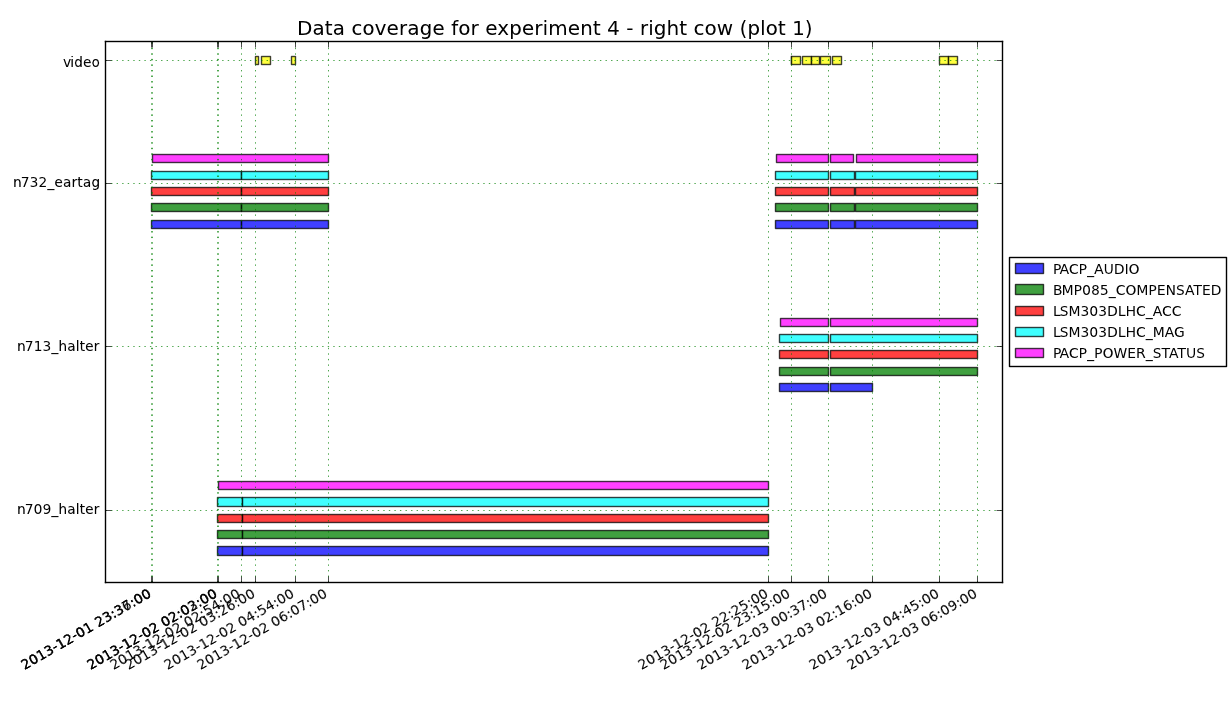
\includegraphics[width=1\textwidth]{images/experiment4_coverage_overall.png}
\end{center}
\caption{Overall coverage of cow in plot 1 in experiment 4}
\label{coverage_plot}
\end{figure}

\begin{figure}[ht!]
\begin{center}
\leavevmode
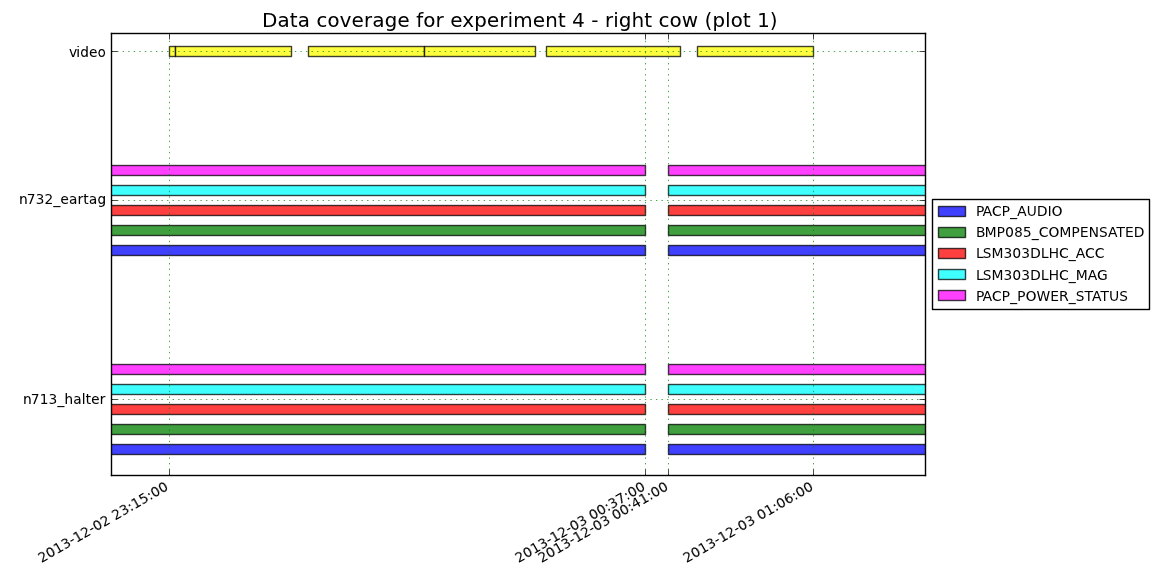
\includegraphics[width=1\textwidth]{images/experiment4_coverage_zoomed.png}
\end{center}
\caption{Overall coverage of cow in plot 1 in experiment 4}
\label{exp4overall}
\end{figure}

Using this figures it was then possible to quickly locate periods where there both signal data and video recordings existed. These periods were then able to be annotated and used for classifier design. 


\section{Data annotation}

In order to create training and test sets so that an algorithm for classification of cow behaviour could be built it was necessary to annotate the recorded signals from the experiments performed. This meant manually looking the recorded data signals, listening to the recorded audio from the sensor nodes and watching the associated video to find individual chew events. To assist with this process, an annotation interface was designed. 

\todo{how annotation is stored in the table}

\subsection{Annotation interface}

To streamline the process of annotating the large amounts of data recorded, an annotation interface was needed to be built. When designing the interface it was important to allow a view of each of the different signals captured. It was also important to do this modularly so that the interface could be used with more or less signals in the future. 

The block diagram in \ref{annotation_interface_design} shows the initial design of the interface. 

\todo{put in a 'design' of the interface'}

To mesh well with the existing code base and for quick prototyping and cross compatibility, the annotation graphical user interface was written using python. Because much of the interface would involve displaying signal data in the way of plots, the matplotlib library was used to assist with the creation of the interface. As well as containing the tools to allow for creating data plots the matplotlib library contains widgets (for example, buttons or selector items) that can be used to make plots more dynamic. 

The inbuilt matplotlib SpanSelector widget was used in the interface so that a very simple click and drag selection process could be used to select sections of data. This allows a user to select a section of data. When done, the start and end time of the selected period is displayed in the interface. The interface also contains a selector widget that allows the user to choose between different event categories to annotate, specifically either 'chew' or 'not chew'. Finally, the interface contains a button that allows the user to submit the annotation. A submitted annotation is stored in the HDF data structure discussed in section \ref{data curation - annotation}. 

The interface also contains functionality to play a selected period of audio. This was enabled by the \texttt{scikits.audiolab} python library \todo{put a reference to audiolab here}. Because of the limitations of this library and the way that it interfaces with the Mac Core Audio library, this only allowed for audio to be played at the standard sampling rate of 44.1 kHz. Fortunately, the audio recorded as part of the experiments that were used was at approximately 22 kHz so it was possible to oversample the audio at double the rate in order to play it. In this case, as the audio is only used to find the start and end of an annotation period, the precise playback frequency is not of great importance. 

The audio playing functionality is implemented in the interface as a play button that plays the audio associated with the 

A user of the annotation interface is then able to select a node, a time period and a range of sensors to be displayed in the interface. Events can then be found within that time period and the audio can be used to precisely find the start and end times. 

\todo{not here but need somewhere explaining what the videos look like}

\todo{add code to appendix and reference}

- annotations stored in the h5 dataset


\subsection{Training set building}

- 3 modes: chew, bite, other
- built annotation interface using matplotlib
	- allows sections to be selected, a mode to be chosen and then allowed for that to be submited through RESTful interface to the server
- also allowed for the audio to be saved
- shows the time in the same format as what is displayed in the video

- using this was able to annotate a lot of the data to build training set of events
- lots of code written to assist with this general extraction

\section{Classifier design}

\subsection{Selection of machine learning algorithm}

Put a table here?

SVM - easy to use, fast to converge, easy to use on embedded systems, something about how to avoids over fitting

ANN - doesn't always converge, 

%%paper with stuff about ML algos for emebedded systems %%http://nesl.ee.ucla.edu/courses/ee202a/shared/samples/projects/2008f/Adam_Stoelting.pdf%%

choice of software package to use too?

matlab - not free but easy to prototype
python - os/workflow already in python/somewhat easy to prototype/good libraries avaliable
C - what an algorithm would eventually implemented in on device, hard to prototype and quickly change things


\section{Classifier evaluation}
